\documentclass[
Karos,
%Loesung,
%Punkte
]{pruefung}

\renewcommand{\Pruefungsfach}{\textbf{Prüfungsfach: Mathematik 2}}
\renewcommand{\Semester}{\textbf{Wintersemester 23/24}}
\renewcommand{\Studiengaenge}{\textbf{Studiengang: WKB}}
\renewcommand{\Fachnummern}{\textbf{Prüfungsnummer: IT 105 20 20}}
\renewcommand{\Dauer}{\textbf{Zeit: 90 Minuten}}
\renewcommand{\Dozenten}{\textbf{Dozent: Karsten Runge}}

\renewcommand{\Hilfsmittel}{
\textbf{Manuskript\newline
 Literatur \newline
 Taschenrechner Casio FX-87DE Plus / Casio FX-87DE Plus 2nd edition}
}
\renewcommand{\Hinweise}{
\textbf{Bearbeiten Sie die Aufgaben ausschließlich auf diesen Prüfungsblättern.
\newline
Begründen Sie alle Lösungsschritte.}
}

\begin{document}
\begin{Aufgabe}[10]
Hinweis: Alle Teilaufgaben können unabhängig voneinander bearbeitet werden.

\begin{enumerate}
	\item
		Ordnen Sie den Differenzialgleichungen die Richtungsfelder zu:
		
		\begin{tabular}{p{0.25\textwidth}p{0.25\textwidth}p{0.25\textwidth}p{0.25\textwidth}}
			(A) $\displaystyle y' = \frac{x}{y}$ &
			(B) $\displaystyle y' = \frac{y}{x}$ &
			(C) $\displaystyle y' = -\frac{x}{y}$ &
			(D) $\displaystyle y' = -\frac{y}{x}$ \\
		\end{tabular}
		
		\begin{tabular}{llll}
			\ifLoesung
			( {\textcolor{red}C} ) &
			\else
			( \quad ) &
			\fi
			\hspace*{-10mm} \raisebox{-0.8\height}{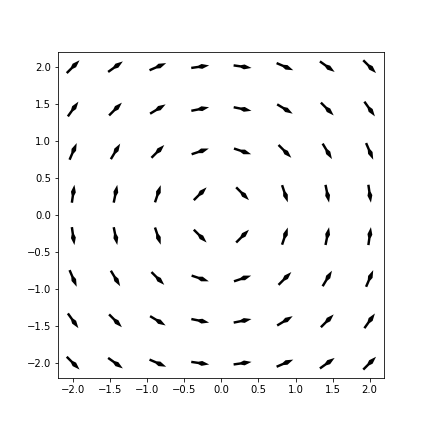
\includegraphics[width=0.4\textwidth]{../M2_IT/m2_it_ws_23_kurzaufgaben_richtungsfeld_3.png}} &
			\ifLoesung
			( {\textcolor{red}D} ) &
			\else
			( \quad ) &
			\fi
			\hspace*{-10mm} \raisebox{-0.8\height}{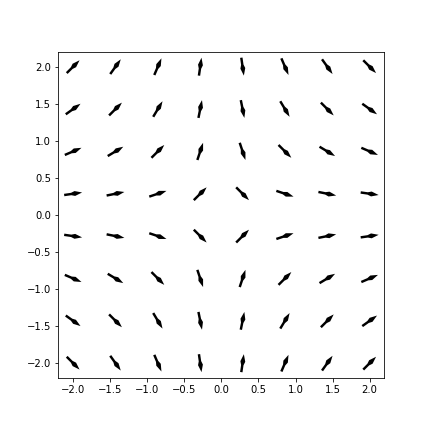
\includegraphics[width=0.4\textwidth]{../M2_IT/m2_it_ws_23_kurzaufgaben_richtungsfeld_4.png}}  \\
			\ifLoesung
			( {\textcolor{red}B} ) &
			\else
			( \quad ) &
			\fi
			\hspace*{-10mm} \raisebox{-0.8\height}{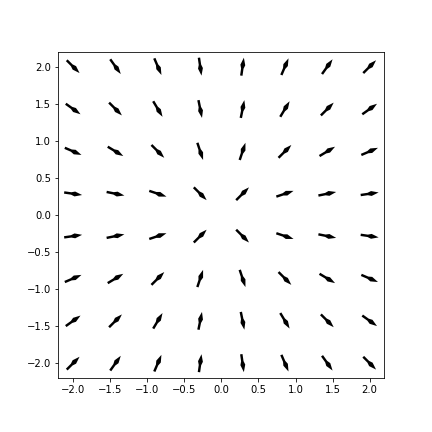
\includegraphics[width=0.4\textwidth]{../M2_IT/m2_it_ws_23_kurzaufgaben_richtungsfeld_2.png}} &
			\ifLoesung
			( {\textcolor{red}A} ) &
			\else
			( \quad ) &
			\fi
			\hspace*{-10mm} \raisebox{-0.8\height}{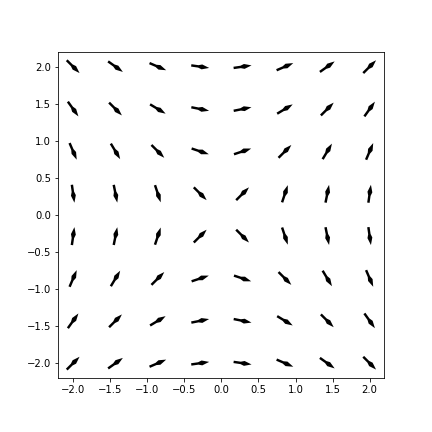
\includegraphics[width=0.4\textwidth]{../M2_IT/m2_it_ws_23_kurzaufgaben_richtungsfeld_1.png}}  \\
		\end{tabular}
		
		\ifLoesung
		\mbox{}\hfill\Punkte{2 P}\\
		\fi	
		
		\pagebreak
	\item
		Bestimmen Sie die allgemeine Lösung der Differenzialgleichung
		\[
			y'(x) = 3 \, x^2 \, y \, .
		\]
		
		\Loesung{10cm}{
			Separation:
			\hfill\Punkte{1 P}
			\[
				\frac{\mathrm{d} \, y}{\mathrm{d} \, x} = 3 \, x^2  \, y 
				\quad \Longrightarrow \quad
				\frac{1}{y} \, \mathrm{d} \, y = 3 \, x^2 \, \mathrm{d} \, x \, .
			\]
			Integration:
			\hfill\Punkte{1 P}
			\[
				\int \frac{1}{y} \, \mathrm{d} \, y = \int 3 \, x^2 \, \mathrm{d} \, x 
				\quad \Longrightarrow \quad
				\ln \left| y \right| = x^3 + C_1, \quad C_1 \in \mathbb{R} \, .
			\]
			Nach $y$ auflösen:
			\hfill\Punkte{1 P}
			\[
				\left| y \right|  = \e^{x^3 + C_1}
				\quad \Longrightarrow \quad
				y = \pm \e^{x^3 + C_1} = \pm \e^C_1 \, \e^{x^3} = C_2 \, \e^{x^3}, \quad C_2 \in \mathbb{R} \, .
			\]
		}
		
	\item
		Berechnen Sie für die Lösung des Anfangswertproblems
		\[
			y'(x) = \frac{y}{1 + x^2}, \quad y(1) = 3 \, ,
		\]
		einen Näherungswert, indem Sie einen Schritt mit dem Euler-Polygonzugverfahren mit der Schrittweite $h=0.2$ durchführen.
		
		\Loesung{}{
			Euler-Polygonzugverfahren:
			\[
			x_1 = x_0 + h = 1.2, 
			\quad
			\tilde{y}_1 = 
			\tilde{y}_0 + h \cdot  \frac{\tilde{y}_0 }{1 + x_0^2} = 
			3 + 0.2 \cdot  \frac{3}{1 + 1^2} = 3.3 \, .
			\hfill\Punkte{2 P}
			\]
		}
		
		\newpage
		
	\item
		Beurteilen Sie den folgenden Dialog mit ChatGPT 3.5.
		Sind die Berechnungen und die Behauptungen von ChatGPT korrekt?
		 
		 \vspace*{2ex}
		 
		 \textbf{You}
		 
		Bitte erstelle ein Beispiel für ein lineares Differenzengleichungssystem mit zwei Unbekannten, das asymptotisch stabil ist.
		
		\vspace*{2ex}
		
		\textbf{ChatGPT}
		
		Betrachten wir das folgende lineare Differenzengleichungssystem mit zwei Unbekannten:
		\[
			\begin{array}{lcl}
				x_{k+1} & = & 0.8 \, x_k + 0.2 \, y_k \\
				y_{k+1} & = & 0.4 \, x_k + 0.6 \, y_k
			\end{array}
		\]
		Die obigen Gleichungen können in Matrixform geschrieben werden als:
		\[
			\left(
				\begin{array}{c}
					x_{k+1} \\
					y_{k+1}
				\end{array}
			\right)
			= 
			\left(
			\begin{array}{cc}
				0.8 & 0.2 \\
				0.4 & 0.6
			\end{array}
			\right)
			\left(
			\begin{array}{c}
				x_{k} \\
				y_{k}
			\end{array}
			\right), \mbox{ mit der Matrix }
			\mathbf{A} =
			\left(
			\begin{array}{cc}
				0.8 & 0.2 \\
				0.4 & 0.6
			\end{array}
			\right)
		\]
		Die Matrix $\mathbf{A}$ ist die Übertragungsmatrix des Systems.
		Um die asymptotische Stabilität zu überprüfen, betrachten wir die Eigenwerte dieser Matrix.
		Die Eigenwerte $\lambda$ können durch das Lösen der charakteristischen Gleichung gefunden werden:
		\[
			\left|
				\begin{array}{cc}
					0.8 - \lambda & 0.2 \\ 
					0.4 & 0.6 - \lambda
				\end{array}
			\right| = 0
			\quad \Longleftrightarrow \quad
			(0.8 - \lambda)(0.6 - \lambda) -0.2 \cdot 0.4 = 0
			\quad \Longleftrightarrow \quad
			\lambda^2 - 1.4 \, \lambda + 0.4 = 0
		\]
		Die Lösungen dieser quadratischen Gleichung sind $\lambda_1=1$ und $\lambda_2=0.4$.
		Beide Eigenwerte haben Beträge kleiner als $1$, was darauf hinweist, dass  das System asymptotisch stabil ist.
		In diesem Beispiel konvergieren die Lösungen für $x_k$ und $y_k$ gegen Null, was auf eine asymptotische Stabilität hinweist.  
		
		\Loesung{}{
			Die Berechnungen sind korrekt.
			Das System ist jedoch nicht asymptotisch stabil, denn der Betrag des Eigenwerts $\lambda_1 = 1$ ist nicht echt kleiner $1$.
			Deshalb konvergieren auch nicht alle Lösungen gegen Null.
			Beispielsweise ist $x_0=1$ und $y_0=1$ ein Fixpunkt. 
			\hfill\Punkte{3 P}
		}
			
	\end{enumerate}
	
\end{Aufgabe}

\newpage

\endinput
\begin{Aufgabe}[9]
	Bestimmen Sie die allgemeine reelle Lösung der Differenzialgleichung
	\[
		y''(x)+ 4 \, y(x) = 8 \, \cos(2 \, x) - 4 \, \sin(2 \, x) \, .
	\]
	
	\Loesung{}{
		Charakteristische Gleichung der homogenen  Differenzialgleichung:
		\hfill\Punkte{2 P}
		\[
			\lambda^2 + 4 = 0
			\quad \Longrightarrow \quad
			\lambda^2 = -4 
			\quad \Longrightarrow \quad
			\lambda = \pm 2 \, \mbox{i} \, .
		\]
		Allgemeine Lösung der homogenen  Differenzialgleichung:
		\hfill\Punkte{1 P}
		\[
			y_h(x) = C_1 \, \cos(2 \, x) + C_2 \, \sin(2 \, x) \, .
		\]
		Ansatz für partikuläre Lösung mit Resonanz:
		\hfill\Punkte{1 P}
		\[
			y_p(x) = x ( A \, \cos(2 \, x) + B \, \sin(2 \, x) ) \, .
		\]
		Erste Ableitung:
		\hfill\Punkte{1 P}
		\[
			y'_p(x) = A \, \cos(2 \, x) + B \, \sin(2 \, x) )+x \, ( - 2\, A \, \sin(2 \, x) + 2 \, B \, \cos(2 \, x) ) \, .
		\]
		Zweite Ableitung:
		\hfill\Punkte{1 P}
		\[
			y''_p(x) = -2 \, A \, \sin(2 \, x) + 2 \, B \, \cos(2 \, x) ) - 2\, A \, \sin(2 \, x) + 2 \, B \, \cos(2 \, x) + x \, ( - 4\, A \, \cos(2 \, x) - 4 \, B \, \sin(2 \, x) )\, .
		\]
		In Differenzialgleichung einsetzen:
		\hfill\Punkte{1 P}
		\begin{eqnarray*}
			\underbrace{-4 \, A \, \sin(2 \, x) + 4 \, B \, \cos(2 \, x) + x \, ( - 4\, A \, \cos(2 \, x) - 4 \, B \, \sin(2 \, x) )}_{\displaystyle y''(x)} & + & 4 \, \underbrace{x ( A \, \cos(2 \, x) + B \, \sin(2 \, x)) }_{\displaystyle y(x)} \\
			& = & 8 \, \cos(2 \, x) - 4 \, \sin(2 \, x) \, .
		\end{eqnarray*}
		Koeffizientenvergleich:
		\hfill\Punkte{1 P}
		\[
			A = 1, \quad B = 2 \, .
		\]
		Allgemeine Lösung:
		\hfill\Punkte{1 P}
		\[
			y(x) = y_h(x) + y_p(x) = C_1 \, \cos(2 \, x) + C_2 \, \sin(2 \, x) + x ( \cos(2 \, x) + 2 \, \sin(2 \, x) ) \, .
		\]
	}
	
	\ifLoesung
	\else
	\newpage
	
	\Loesung{}{}
	\fi
	
\end{Aufgabe}

\newpage

\endinput
\begin{Aufgabe}[10]% Siehe SS 16
	Bestimmen Sie die allgemeine reelle Lösung des Differenzialgleichungssystems
	\[
	\begin{array}{ccrcrcr}
		\dot{x}_1 & = & -2 \, x_1 & + & 3 \, x_2 & + & 6 \, \e^{-2 \, t} \, ,\\
		\dot{x}_2 & = &  2 \, x_1 &  + & 3 \, x_2 & .   &  \\
	\end{array}
	\]
	
	\Loesung{}{
		Matrixform:
		\hfill\Punkte{1 P}
		\[
		\dot{\mathbf{x}}
		=
		\left(
		\begin{array}{rr}
			-2 & 3\\
			2 &  3\\
		\end{array}
		\right)
		\mathbf{x} +
		\left(
		\begin{array}{c}
			 6 \, \e^{-2 \, t}\\
			0\\
		\end{array}
		\right)
		\, .
		\]
		Eigenwerte:
		\hfill\Punkte{2 P}
		\[
		\left|
		\begin{array}{cc}
			-2-\lambda &            3\\
			2                & 3 - \lambda\\
		\end{array}
		\right|
		=(-2-\lambda)(3-\lambda)-3 \cdot 2 = \lambda^2-\lambda-12 = 0
		\, \Longrightarrow \,
		\lambda_{1,2} = \frac{1\pm\sqrt{1+48}}{2} = 4 | -3 \, .
		\]
		Eigenvektor $\mathbf{v}_1$ zu $\lambda_1=4$:
		\hfill\Punkte{1 P}
		\[
		\left(
		\begin{array}{cc}
			-2-4 &                 3\\
			2                     & 3-4\\
		\end{array}
		\right)
		\mathbf{v}_1
		=
		\left(
		\begin{array}{rr}
			-6 &  3\\
		 2  & -1\\
		\end{array}
		\right)
		\mathbf{v}_1
		= \mathbf{0}
		\quad \Longrightarrow \quad
		\mathbf{v}_1
		=
		\left(
		\begin{array}{c}
			1\\
			2\\
		\end{array}
		\right) \, .
		\]
		Eigenvektor $\mathbf{v}_2$ zu $\lambda_2=-3$:
		\hfill\Punkte{1 P}
		\[
		\left(
		\begin{array}{cc}
			-2+3 &                 3\\
			2                     & 3+3\\
		\end{array}
		\right)
		\mathbf{v}_2
		=
		\left(
		\begin{array}{cc}
			1 &  3\\
			2  & 6\\
		\end{array}
		\right)
		\mathbf{v}_2
		= \mathbf{0}
		\quad \Longrightarrow \quad
		\mathbf{v}_2
		=
		\left(
		\begin{array}{r}
			3\\
			-1\\
		\end{array}
		\right) \, .
		\]
		Allgemeine reelle Lösung des homogenen Differenzialgleichungssystems:
		\hfill\Punkte{1 P}
		\[
		\mathbf{x}_h
		= C_1 \, \e^{4 \, t}\
		\left(
		\begin{array}{c}
			1\\
			2\\
		\end{array}
		\right)
		+ C_2 \, \e^{- 3 \, t}
		\left(
		\begin{array}{r}
		 3\\
			-1\\
		\end{array}
		\right),
		\quad C_1, C_2\in \mathbb{R} \, .
		\]
	}
	
	\newpage
	
	\Loesung{}{
		Ansatz für partikuläre Lösung ohne Resonanz:
		\hfill\Punkte{1 P}
		\[
			\mathbf{x}_p
			= \e^{- 2 \, t}\
			\left(
			\begin{array}{c}
				A\\
				B\\
			\end{array}
			\right) \, .
		\]
		Ableitung in Differenzialgleichungssystem eingesetzt:
		\hfill\Punkte{1 P}
		\[
			-2 \, \e^{- 2 \, t}\
			\left(
			\begin{array}{c}
				A\\
				B\\
			\end{array}
			\right)
			=
			\left(
			\begin{array}{rr}
				-2 & 3\\
				2 &  3\\
			\end{array}
			\right)
			\e^{- 2 \, t}\
			\left(
			\begin{array}{c}
				A\\
				B\\
			\end{array}
			\right) +
			\left(
			\begin{array}{c}
				6 \, \e^{-2 \, t}\\
				0\\
			\end{array}
			\right)
			\, .
		\]
		Lineares Gleichungssystem:
		\hfill\Punkte{1 P}
		\[
			\begin{array}{rcrcrcr}
				-2 \, A & = & -2 \, A & + & 3 \, B & + & 6 \\
				-2 \, B & = &   2 \, A & + & 3 \, B &    & \\
			\end{array}
			\quad \Longrightarrow \quad
			B = -2, \, A = 5 \, .
		\]
		Allgemeine reelle Lösung des Differenzialgleichungssystems:
		\hfill\Punkte{1 P}
		\[
			\mathbf{x} = \mathbf{x}_h + \mathbf{x}_p
			= C_1 \, \e^{4 \, t}\
			\left(
			\begin{array}{c}
				1\\
				2\\
			\end{array}
			\right)
			+ C_2 \, \e^{- 3 \, t}
			\left(
			\begin{array}{r}
				3\\
				-1\\
			\end{array}
			\right) +
			e^{- 2 \, t}
			\left(
			\begin{array}{r}
				 5\\
				-2\\
			\end{array}
			\right),
			\quad C_1, C_2\in \mathbb{R} \, .
		\]
	}
	
\end{Aufgabe}

\newpage

\endinput
\begin{Aufgabe}[8] 
	Eine Differenzengleichung erster Ordnung ist gegeben durch
	\[
		x_{k+1} = 1.05 \, x_k - 1, \quad x_0 = 10, \quad k = 0,1,2,3,\ldots . 
	\]
	\begin{enumerate}
		\item
			Geben Sie die Zahlenwerte von $x_1$ und $x_2$ an.
		\item
		  	Bestimmen Sie die Lösung der Differenzengleichung.
		 \item
		 	Für welche Indizes $k$ ist $x_k < 0$?  
	\end{enumerate}
	
	\Loesung{}{
		\begin{enumerate}
			\item
				Zahlenwerte:
				\hfill\Punkte{1 P}
				\[
					x_0 = 1.05 \cdot 10 - 1 = 9.5, \quad x_1 = 1.05 \cdot 9.5 - 1 = 8.975
				\]
			\item
				Lösungsformel:
				\hfill\Punkte{1 P}
				\[
					x_{k+1} = \lambda \, x_k + r_k
					\quad \Longrightarrow \quad
					x_k = \lambda^k \cdot x_0 + \sum_{l=0}^{k-1} \lambda^{k-1-l} r_l \, .
				\]
				$\lambda = 1.05$, $r_k = -1$, $x_0 = 1$:
				\hfill\Punkte{1 P}
				\[
					x_k = 1.05^k \cdot 10 + \sum_{l=0}^{k-1}1.05^{k-1-l} \cdot (-1) \, .
				\]
				Geometrische Reihe:
				\hfill\Punkte{1 P}
				\[
					x_k =
					1.05^k \cdot 10 - \frac{1 - 1.05^k}{1 - 1.05} \, .
				\]
				Vereinfachung:
				\hfill\Punkte{1 P}
				\[
					x_k =
					10 \cdot 1.05^k  - \frac{1 - 1.05^k}{- 0.05} =
					10 \cdot 1.05^k  + 20 - 20 \cdot 1.05^k =
					- 10 \cdot 1.05^k  + 20\, .
				\]
			\item
				Bedingung $x_k < 0$:
				\hfill\Punkte{1 P}
				\[
					- 10 \cdot 1.05^k  + 20 < 0
					\quad \Longleftrightarrow \quad
					20 < 10 \cdot 1.05^k
					\quad \Longleftrightarrow \quad
					2 < 1.05^k \, .
				\]
				Nach $k$ auflösen:
				\hfill\Punkte{1 P}
				\[
					\ln(2) < \ln\left((1.05)^k\right)
					\quad \Longleftrightarrow \quad
					\ln(2) < k \, \ln(1.05)
					\quad \Longleftrightarrow \quad
					k > \frac{\ln(2)}{\ln(1.05)} \approx 14.2
				\]
				Ab $k = 15$ sind alle Folgenglieder negativ.
				\hfill\Punkte{1 P}
		\end{enumerate}
	}
	
	\newpage
	
	\Loesung{}{
		Alternative Lösung für \textbf{b)}
		\par
		\vspace*{1cm}
		\par
		Homogene Lösung:
		\[
			x_{k+1} -1.05 \, x_k = 0
			\quad \Longrightarrow \quad
			\lambda - 1.05 = 0
			\quad \Longrightarrow \quad
			\lambda = 1.05
			\quad \Longrightarrow \quad
			x_k^h = C \cdot 1.05^k \, .
		\]
		Partikuläre Lösung
		\[
			x_k^p = A
			\quad \Longrightarrow \quad
			A - 1.05 \, A = - 1
			\quad \Longrightarrow \quad
			A ( 1 - 1.05 ) = -1
			\quad \Longrightarrow \quad
			A = \frac{-1}{-0.05} = 20 \, .
		\]
		Allgemeine Lösung:
		\[
			x_k = x_k^h + x_k^p = C \cdot 1.05^k + 20 \, .
		\]
		Anfangswert $x_0 = 10$: 
		\[
			k = 0: \quad 
			x_0 = C \cdot 1.05^0 + 20 
			\quad \Longrightarrow \quad
			10 = C + 20
			\quad \Longrightarrow \quad
			C = -10 \, .
		\]
		Ergebnis:
		\[
			x_k = -10 \cdot 1.05^k + 20 \, .
		\]
	}
	
\end{Aufgabe} 

\newpage

\endinput
\begin{Aufgabe}[8] 
	Die Geschwister Fin und Ans haben ein Baugrundstück geerbt und planen darauf ein Gebäude mit 10 Mietwohnungen errichten zu lassen. Sie können zusammen ein Eigenkapital von 500.000 Euro aufbringen, der Rest muss über einen Kredit finanziert werden.
	\begin{enumerate}
		\item Aufgrund stark gestiegener Kreditzinsen könnte der Bau von Sozialwohnungen eine attraktive Möglichkeit darstellen. Durch staatliche Förderung liegt der Zinssatz hier bei $1.2 \%$ p.a. bei unterjähriger, genauer monatlicher Verzinsung, d.h. der Zinssatz je Monat liegt bei $0.1 \%$. \\
		Der Bau der $10$ Wohnungen soll 1.5 Millionen Euro kosten, es muss also 1 Million Euro Kredit aufgenommen werden.
		\begin{itemize}
			\item Bestimmen Sie den effektiven Jahreszins (auf zwei Nachkommastellen genau).
			\item Welche Rate R muss jeweils zum Ende des Monats gezahlt werden, damit der Kredit nach genau 20 Jahren (also 240 Monaten) getilgt ist? \\
			Hinweis: Sie können z.B. die Zahlung der 240 Raten als konstante Zahlungsfolge betrachten, deren Barwert oder Endwert mit einem geeigneten Wert gleich zu setzen ist.
			\item Welche monatliche Kaltmiete muss für jede der 10 Wohnungen erhoben werden, damit aus den Mieteinnahmen die Kreditraten R beglichen werden können? Dabei sollen zusätzliche Kosten für Instandhaltung oder Steuern vernachlässigt werden.
		\end{itemize}
		\item Werden Wohnungen für den freien Markt gebaut, sind die Zinsen wesentlich höher. Sie liegen bei $4.8\%$ p.a. bei monatlicher Verzinsung. Zusätzlich werden höhere Baukosten von 2 Millionen Euro (also ein Kredit von 1.5 Millionen Euro) eingeplant, um einen erhöhten Wohnkomfort zu erreichen.
		\begin{itemize}
			\item Bestimmen Sie den effektiven Jahreszins (auf zwei Nachkommastellen genau).
			\item Welche Rate R muss jeweils zum Ende des Monats gezahlt werden, damit der Kredit nach genau 20 Jahren getilgt ist?
			\item Welche monatliche Kaltmiete muss für jede der 10 Wohnungen erhoben werden, damit aus den Mieteinnahmen die Kreditraten R beglichen werden können?
		\end{itemize} 
	\end{enumerate}
\end{Aufgabe}
\Loesung{}{
\textbf{a)}
effektiver Jahreszins $p^*=100\cdot((1+\frac{1.2}{12\cdot 100})^{12}-1)\approx 1.21$
\hfill\Punkte{1 P}\\\\
Der Barwert der Zahlung aller 240 Raten R liegt bei 1 Million Euro. Deswegen kann man setzen \hfill\Punkte{2 P}
\[R\cdot (\frac{1}{1.001}+\frac{1}{1.001^2}+...+\frac{1}{1.001^{240}})=1000000\]
Multiplikation der Gleichung mit $1.001^{240}$ ergibt
\[R\cdot (1.001^{239}+1.001^{238}+...+1)=1000000\cdot 1.001^{240}\]
Die Anwendung der geometrischen Summenformel führt zu 
\[R\cdot \frac{1.001^{240}-1}{1.001-1}=1000000\cdot 1.001^{240}\]
Damit ist \[R= 10000\cdot \frac{1.001^{240}}{1.001^{240}-1}\approx 4688.72 (\text{Euro)}\]

}
\newpage
\Loesung{}{

monatliche Kaltmiete: \hfill\Punkte{1 P}
\[4688.72:10\approx 468.88 \text{\;(Euro)}\]
Hier muss aufgerundet werden.\\
\textbf{b)}
effektiver Jahreszins $p^*=100\cdot((1+\frac{4.8}{12\cdot 100})^{12}-1)\approx 4.91$ \hfill\Punkte{1 P}\\\\
Der Barwert der Zahlung aller 240 Raten R liegt bei 1.5 Million Euro. Deswegen kann man (bei monatlichen Zinsen von $0.4\%$) setzen \hfill\Punkte{2 P}
\[R\cdot (\frac{1}{1.004}+\frac{1}{1.004^2}+...+\frac{1}{1.004^{240}})=1500000\]
Die geometrische Summenformel und Umstellen nach R ergibt
\[R= 1500000\cdot 0.004\cdot \frac{1.004^{240}}{1.004^{240}-1}\approx 9734.36 \text{\;(Euro)}\]
monatliche Kaltmiete: \hfill\Punkte{1 P}
\[9734.36:10\approx 973.44\text{\;(Euro)}\]
}
\ifLoesung
\else
\newpage
\Loesung{}{}
\fi

\newpage

\endinput
%\begin{Aufgabe}[2] 
	Finanzmathematik II
\end{Aufgabe}

\newpage

\endinput
\begin{Aufgabe}[9]

Gegeben ist das lineare Optimierungsproblem 
\[ 
f(\vec x)=\vec c\cdot \vec x\stackrel{!}{=}\mathrm{Max}, \quad \mathbf A\vec x\leq \vec b,\quad \vec x\geq 0, 
\] 
mit 
\[ 
\vec    c = \left(\begin{array}{c}  -1\\ 2 \end{array}\right),\quad 
\mathbf A = \left(\begin{array}{cc} -1 & 1\\ 1 & 1\\ 1 & 0 \end{array}\right),\quad 
\vec    b = \left(\begin{array}{c}  1\\ 5\\ 3 \end{array}\right)\,. 
\] 

\begin{enumerate}
	\item 	Zeichnen Sie den zulässigen Bereich in das gegebene Koordinatensystem ein.
	\item 	Zeichnen Sie im zulässigen Bereich alle Punkte $(x_1,x_2)$ mit 
	$f(x_1,x_2)=1$ ein. 
	\item 	Wenden Sie den Primalen Simplex-Algorithmus auf das lineare Optimierungsproblem an.
\end{enumerate}

\begin{center} 
	\begin{tikzpicture}[xscale=1,yscale=1] 
		\draw[help lines,step=0.5] (-5.5,-1.0) grid (12.0,9.0); 
		\draw[->, darkgray, line width=1pt] (-1.5,0) -- (5.5,0) node[below] {$x_1$}; 
		\draw[->, darkgray, line width=1pt] (0,-1.0) -- (0,6.5) node[left] {$x_2$}; 
		\foreach \i in {-1,...,-1} { \draw (\i,0.1) -- (\i,-0.1) node[below] {$\i$}; } 
		\foreach \i in {1,...,5} { \draw (\i,0.1) -- (\i,-0.1) node[below] {$\i$}; } 
		\foreach \i in {1,...,6} { \draw (0.1,\i) -- (-0.1,\i) node[left] {$\i$}; } 
		\foreach \i in {-1,...,-1} {\draw (0.1,\i) -- (-0.1,\i) node[left] {$\i$};} 
		\ifLoesung 
		\coordinate[] (P) at (0,1); \fill (P) circle (2pt); 
		\coordinate[label=] (Q) at (3,0); \fill (Q) circle (2pt); 
		\coordinate[label=] (R) at (0,0); \fill (R) circle (2pt); 
		\coordinate[label= ] (S) at (2,3); \fill (S) circle (2pt); 
		\coordinate[label= ] (T) at (3,2); \fill (T) circle (2pt); 
		\coordinate[label= right: Zulässigkeitsbereich  ] (S1) at (0.0,0.25);  
		\coordinate[label= right: Isolinie ] (S2) at (2,1.5); 
		
		\draw[ultra thick,-] (0,1)--(2,3); 
		\draw[ultra thick,-] (2,3)--(3,2); 
		\draw[ultra thick,-] (3,0)--(3,2);
		\draw[ultra thick,-] (0,0)--(3,0); 
		\draw[ultra thick,-] (0,0)--(0,1); 
		\draw[gray, dashed, ultra thick,-] (0,0.5)--(3,2); 
		\fi
	\end{tikzpicture} 
\end{center} 

\clearpage
\Loesung{}{
	
	% ----------------------------------------------------------------------------
	% MATLAB-Quelltext
	% p  = 5;
	% K0 = 30000;
	% N1 = -K0 + 15000/(1+p/100) + 17000/(1+p/100)^2
	% N2 = -K0 + 16500/(1+p/100) + 16000/(1+p/100)^2
	% K2 = K0*(1+5/(12*100))^(12*2)
	% pstern= 100*((1+p/(12*100))^12-1)
	% ----------------------------------------------------------------------------
	
	\begin{enumerate}
		\item Zulässigkeitsbereich: siehe Skizze. 				
		\hfill\Punkte{2} 
		
		\item Isolinie $f(x_1,x_2)=1$: siehe Skizze.			
		\hfill\Punkte{1}
		
		\item 
		Das LOP ist in Standardformat gegeben und wegen $\vec 0 \leq \vec b$ ist $\vec 0$ ein Eckpunkt des zulässigen Bereichs. \\ 
		Das Ausgangstableau lautet 
		\[ 
		\begin{array}{c|cc|ccc|c} 
			\mbox{BV} &  x_1                   & x_2                    & z_1                    & z_2                    & z_3                    & b_i  \\ \hline 
			z_1      & -1 & 1 & 1 & 0 & 0 & 1  \\ 
			z_2      & 1 & 1 & 0 & 1 & 0 & 5 \\ 
			z_3      & 1 & 0 & 0 & 0 & 1 & 3 \\ \hline 
			f        & -1 & 2 & 0 & 0 & 0 & 0 \\ 
		\end{array} 
		\hfill\Punkte{1}
		\] 
		$1$. Schritt: 
		Pivot-Spalte: $2$; Pivot-Zeile: $1$. Die Nichbasisvariable $x_{2}$ wird in die Basis aufgenommen. Dies führt auf das Tableau 
		\[ 
		\begin{array}{c|cc|ccc|c} 
			\mbox{BV}   &  x_1                    & x_2                     & z_1                     & z_2                     & z_3                     & b_i  \\ \hline 
			x_2 & -1 & 1 & 1 & 0 & 0 & 1\\ 
			z_2 & 2 & 0 & -1 & 1 & 0 & 4\\ 
			z_3  & 1 & 0 & 0 & 0 & 1 & 3\\ \hline 
			f          & 1 & 0 & -2 & 0 & 0 & -2\\ 
		\end{array} 
		\hfill\Punkte{2}
		\] 
		$2$. Schritt: 
		Pivot-Spalte: $1$; Pivot-Zeile: $2$. 
		Die Nichbasisvariable $x_{1}$ wird in die Basis aufgenommen. Dies führt auf das Tableau 
		\[ 
		\begin{array}{c|cc|ccc|c} 
			\mbox{BV}   &  x_1                    & x_2                     & z_1                     & z_2                     & z_3                     & b_i  \\ \hline 
			x_2  & 0 & 1 & \frac{1}{2} & \frac{1}{2} & 0 & 3\\ 
			x_1 & 1 & 0 & -\frac{1}{2} & \frac{1}{2} & 0 & 2\\ 
			z_3  & 0 & 0 & \frac{1}{2} & -\frac{1}{2} & 1 & 1\\ \hline 
			f          & 0 & 0 & -\frac{3}{2} & -\frac{1}{2} & 0 & -4\\ 
		\end{array} 
		\hfill\Punkte{2}
		\] 
		Die Zielfunktionszeile enthält nur Elemente $\leq 0$. Dies entspricht der 1. Abbruchbedingung. \\ 
		Die optimale zulässige Lösung ist $(x_1,x_2)=(2,3)$ mit $f(x_1,x_2)= 4$. 
		\hfill\Punkte{1}
		
		
		
		
		
	\end{enumerate}
	%\smallskip
%	\HFehler{
%		\begin{itemize}
			
%		\end{itemize}
%	}
	
	
}



\ifLoesung
\else
\newpage
\Loesung{}{}
\fi



\end{Aufgabe}

\newpage

\endinput
\end{document}
